\documentclass[tikz,border=2pt]{standalone}
\usepackage{amsmath,amssymb}
\usepackage{tikz}
\usetikzlibrary{arrows.meta}

\begin{document}
% Homogeneity of degree m: moving out along a ray through the origin, from x to 2x to 3x,
% multiplies the value by 2^m and 3^m.
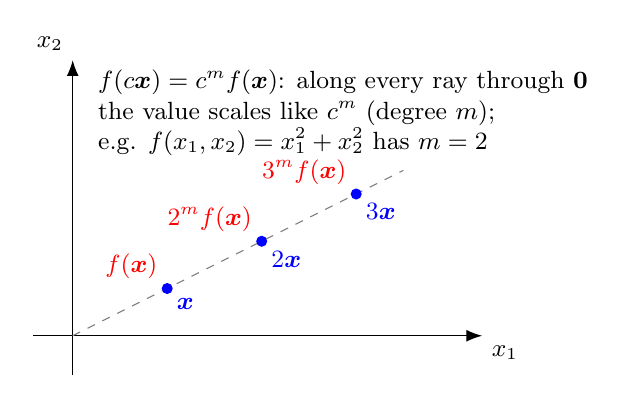
\begin{tikzpicture}[every node/.style={font=\small}, >={Latex[length=2mm]}]
	\draw[->] (-0.5,0) -- (5.2,0) node[below right] {$x_1$};
	\draw[->] (0,-0.5) -- (0,3.5) node[above left] {$x_2$};
	\draw[gray, dashed] (0,0) -- (4.2,2.1);
	\fill[blue] (1.2,0.6) circle (2pt) node[below right] {$\boldsymbol{x}$};
	\fill[blue] (2.4,1.2) circle (2pt) node[below right] {$2\boldsymbol{x}$};
	\fill[blue] (3.6,1.8) circle (2pt) node[below right] {$3\boldsymbol{x}$};
	\node[red, above left, font=\small] at (1.2,0.6) {$f(\boldsymbol{x})$};
	\node[red, above left, font=\small] at (2.4,1.2) {$2^m f(\boldsymbol{x})$};
	\node[red, above left, font=\small] at (3.6,1.8) {$3^m f(\boldsymbol{x})$};
	\node[anchor=north west, align=left] at (0.2,3.5) {$f(c\boldsymbol{x})=c^m f(\boldsymbol{x})$: along every ray through $\boldsymbol{0}$\\ the value scales like $c^m$ (degree $m$);\\ e.g. $f(x_1,x_2)=x_1^2+x_2^2$ has $m=2$};
\end{tikzpicture}
\end{document}
